\documentclass[14pt,a4paper]{article}
% chinese
\usepackage{ctex}
\usepackage{CJK}
\usepackage[margin=2.5cm]{geometry}
% graph
\usepackage{pgf}
\usepackage{tikz}
\usetikzlibrary{arrows}
\usetikzlibrary{calc}
\usetikzlibrary{shapes.multipart}
\usetikzlibrary{chains}
\newcommand*\circled[1]{\tikz[baseline=(char.base)]{
            \node[shape=circle,draw,inner sep=1pt] (char) {\bf #1};}}
% math
\usepackage{amsmath}
\usepackage{kbordermatrix}
\DeclareMathOperator{\head}{head}
\DeclareMathOperator{\tail}{tail}
% fancy
\usepackage{fancyhdr}
\pagestyle{fancy}
\lhead{数据结构与算法第四次课后作业}
\rhead{叶鉴赏}

\begin{document}
	\title{\bf 数据结构与算法第四次作业}
	\author{软件工程(软件技术)四班\ 叶鉴赏\ 2016220204004}
	\maketitle
	\tableofcontents
	\newpage

	\section{有向图}
	\begin{center}
		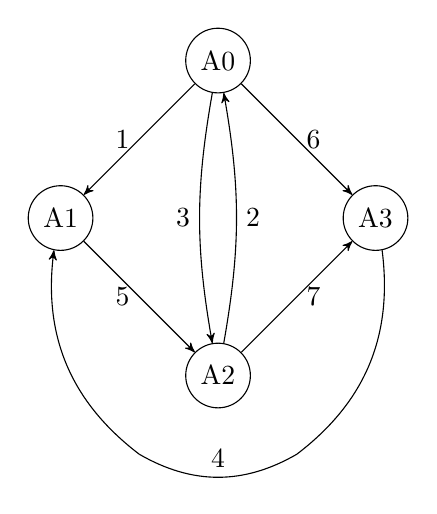
\begin{tikzpicture}[>=stealth',->]
			\node[draw,circle](A0)at(2,4){A0};
			\node[draw,circle](A1)at(0,2){A1};
			\node[draw,circle](A2)at(2,0){A2};
			\node[draw,circle](A3)at(4,2){A3};
			\draw[left](A0)edge node{1}(A1);
			\draw[left](A1)edge node{5}(A2);
			\draw[right](A2)edge node{7}(A3);
			\draw[right](A0)edge node{6}(A3);
			\draw[left,bend right=10](A0)edge node{3}(A2);
			\draw[right,bend right=10](A2)edge node{2}(A0);
			\draw[-,bend left=30](A3)edge node{}(3,-1);
			\draw[-,above,bend left=30](3,-1)edge node{4}(1,-1);
			\draw[bend left=30](1,-1)edge node{}(A1)[-];
		\end{tikzpicture}
	\end{center}

	\subsection{出度、入度}
	\begin{center}
		\begin{tabular}{|c|c|c|}
			\hline
			顶点 & 出度 & 入度 \\
			\hline
			 A0  &  3   &   1  \\
			 A1  &  1   &   2  \\
			 A2  &  2   &   2  \\
			 A3  &  1   &   2  \\
			\hline
		\end{tabular}
	\end{center}
	\subsection{邻接矩阵}
	$$
	\bbordermatrix{
		       & \rm A0 & \rm A1 & \rm A2 & \rm A3 \cr
		\rm A0 &    0   &    1   &    1   &    1   \cr
		\rm A1 &    0   &    0   &    1   &    0   \cr
		\rm A2 &    1   &    0   &    0   &    1   \cr
		\rm A3 &    0   &    1   &    0   &    0   \cr
	}
	$$
	\subsection{关联矩阵}
	$$
	\bbordermatrix{
		       & 1 & 2 & 3 & 4 & 5 & 6 & 7 \cr
		\rm A0 & -1& 1 & -1& 0 & 0 & -1& 0 \cr
		\rm A1 & 1 & 0 & 0 & 1 & -1& 0 & 0 \cr
		\rm A2 & 0 & -1& 1 & 0 & 1 & 0 & -1\cr
		\rm A3 & 0 & 0 & 0 & -1& 0 & 1 & 1 \cr
	}
	$$

	\subsection{邻接表}
	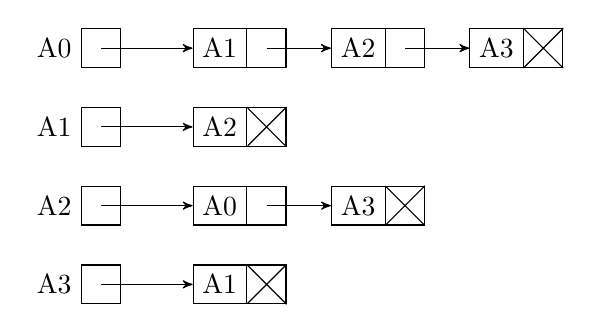
\begin{tikzpicture}[>=stealth',auto]
		\tikzstyle{listhead}=[rectangle,draw,minimum size=14pt];
		\tikzstyle{listnode}=[node distance=50pt,
			rectangle split,rectangle split horizontal,rectangle split parts=2,
			rectangle split part align=center,draw,minimum size=14pt,
			rectangle split empty part width=3pt];
		\node[listhead,label=left:A0](00){};
		\node[listnode,right of=00](01){A1}edge[<-](00.center);
		\node[listnode,right of=01](02){A2}edge[<-](01.two north|-01.two east);
		\node[listnode,right of=02](03){A3}edge[<-](02.two north|-02.two east);
		\draw(03.south east)--+(-14pt,+14pt)(03.north east)--+(-14pt,-14pt);

		\node[listhead,below of=00,label=left:A1](10){};
		\node[listnode,right of=10](11){A2}edge[<-](10.center);
		\draw(11.south east)--+(-14pt,+14pt)(11.north east)--+(-14pt,-14pt);

		\node[listhead,below of=10,label=left:A2](20){};
		\node[listnode,right of=20](21){A0}edge[<-](20.center);
		\node[listnode,right of=21](22){A3}edge[<-](21.two north|-21.two east);
		\draw(22.south east)--+(-14pt,+14pt)(22.north east)--+(-14pt,-14pt);

		\node[listhead,below of=20,label=left:A3](30){};
		\node[listnode,right of=30](31){A1}edge[<-](30.center);
		\draw(31.south east)--+(-14pt,+14pt)(31.north east)--+(-14pt,-14pt);
	\end{tikzpicture}

	\subsection{逆邻接表}
	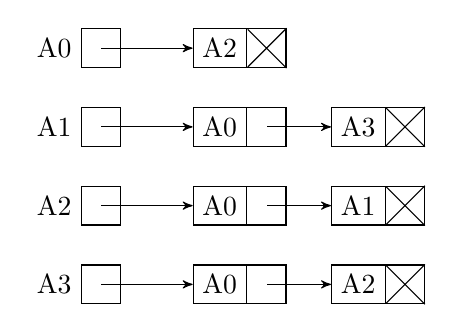
\begin{tikzpicture}[>=stealth',auto]
		\tikzstyle{listhead}=[rectangle,draw,minimum size=14pt];
		\tikzstyle{listnode}=[node distance=50pt,
			rectangle split,rectangle split horizontal,rectangle split parts=2,
			rectangle split part align=center,draw,minimum size=14pt,
			rectangle split empty part width=3pt];
		\node[listhead,label=left:A0](00){};
		\node[listnode,right of=00](01){A2}edge[<-](00.center);
		\draw(01.south east)--+(-14pt,+14pt)(01.north east)--+(-14pt,-14pt);

		\node[listhead,below of=00,label=left:A1](10){};
		\node[listnode,right of=10](11){A0}edge[<-](10.center);
		\node[listnode,right of=11](12){A3}edge[<-](11.two north|-11.two east);
		\draw(12.south east)--+(-14pt,+14pt)(12.north east)--+(-14pt,-14pt);

		\node[listhead,below of=10,label=left:A2](20){};
		\node[listnode,right of=20](21){A0}edge[<-](20.center);
		\node[listnode,right of=21](22){A1}edge[<-](21.two north|-21.two east);
		\draw(22.south east)--+(-14pt,+14pt)(22.north east)--+(-14pt,-14pt);

		\node[listhead,below of=20,label=left:A3](30){};
		\node[listnode,right of=30](31){A0}edge[<-](30.center);
		\node[listnode,right of=31](32){A2}edge[<-](31.two north|-31.two east);
		\draw(32.south east)--+(-14pt,+14pt)(32.north east)--+(-14pt,-14pt);
	\end{tikzpicture}

	\subsection{十字链表}
	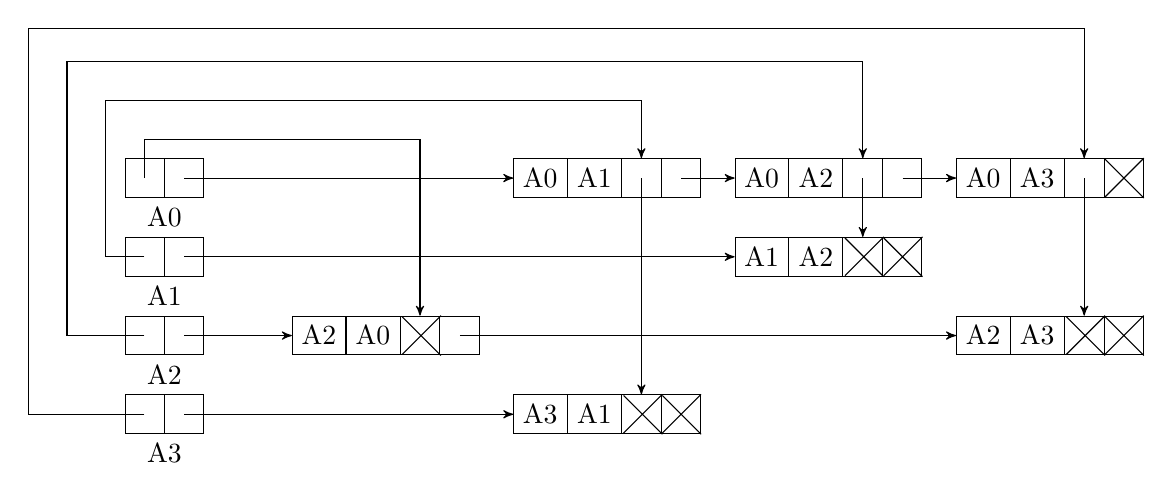
\begin{tikzpicture}[->,>=stealth',auto]
		\tikzstyle{listhead}=[rectangle,rectangle split,
			rectangle split horizontal,rectangle split parts=2,
			rectangle split part align=center,draw,minimum size=14pt,
			rectangle split empty part width=3pt];
		\tikzstyle{listnode}=[node distance=80pt,
			rectangle split,rectangle split horizontal,rectangle split parts=4,
			rectangle split part align=center,minimum size=14pt,
			rectangle split empty part width=3pt];
		\node[listhead,label=below:A0](0){};
		\node[listnode,right of=0](00){};
		\node[listnode,right of=00,draw](01){A0\nodepart{two}A1};
		\node[listnode,right of=01,draw](02){A0\nodepart{two}A2};
		\node[listnode,right of=02,draw](03){A0\nodepart{two}A3};
		\node[listhead,below of=0,label=below:A1](1){};
		\node[listnode,right of=1](10){};
		\node[listnode,right of=10](11){};
		\node[listnode,right of=11,draw](12){A1\nodepart{two}A2};
		\node[listhead,below of=1,label=below:A2](2){};
		\node[listnode,right of=2,draw](20){A2\nodepart{two}A0};
		\node[listnode,right of=20](21){};
		\node[listnode,right of=21](22){};
		\node[listnode,right of=22,draw](23){A2\nodepart{two}A3};
		\node[listhead,below of=2,label=below:A3](3){};
		\node[listnode,right of=3](30){};
		\node[listnode,right of=30,draw](31){A3\nodepart{two}A1};

		\draw(0.two north|-0.two east)--(01);
		\draw(01.four north|-01.four east)--(02);
		\draw(02.four north|-02.four east)--(03);
		\draw[-](03.south east)--+(-14pt,14pt)(03.north east)--+(-14pt,-14pt);
		\draw(1.two north|-1.two east)--(12);
		\draw[-](12.south east)--+(-14pt,14pt)(12.north east)--+(-14pt,-14pt);
		\draw(2.two north|-2.two east)--(20);
		\draw(20.four north|-20.four east)--(23);
		\draw[-](23.south east)--+(-14pt,14pt)(23.north east)--+(-14pt,-14pt);
		\draw(3.two north|-3.two east)--(31);
		\draw[-](31.south east)--+(-14pt,14pt)(31.north east)--+(-14pt,-14pt);

		\draw(0.one north|-0.one east)-|+(0,14pt)-|(20.three north|-20.north east);
		\draw[-]([xshift=-14pt]20.south east)--+(-14pt,14pt)([xshift=-14pt]20.north east)--+(-14pt,-14pt);
		\draw(1.one north|-1.one east)-|+(-14pt,56.5pt)-|(01.three north|-01.north east);
		\draw(01.three north|-01.three east)--(31.three north|-31.north east);
		\draw[-]([xshift=-14pt]31.south east)--+(-14pt,14pt)([xshift=-14pt]31.north east)--+(-14pt,-14pt);
		\draw(2.one north|-2.one east)-|+(-28pt,99pt)-|(02.three north|-02.north east);
		\draw(02.three north|-02.three east)--(12.three north|-12.north east);
		\draw[-]([xshift=-14pt]12.south east)--+(-14pt,14pt)([xshift=-14pt]12.north east)--+(-14pt,-14pt);
		\draw(3.one north|-3.one east)-|+(-42pt,139.5pt)-|(03.three north|-03.north east);
		\draw(03.three north|-03.three east)--(23.three north|-23.north east);
		\draw[-]([xshift=-14pt]23.south east)--+(-14pt,14pt)([xshift=-14pt]23.north east)--+(-14pt,-14pt);
	\end{tikzpicture}

	\newpage
	\section{无向图}
	\begin{center}
		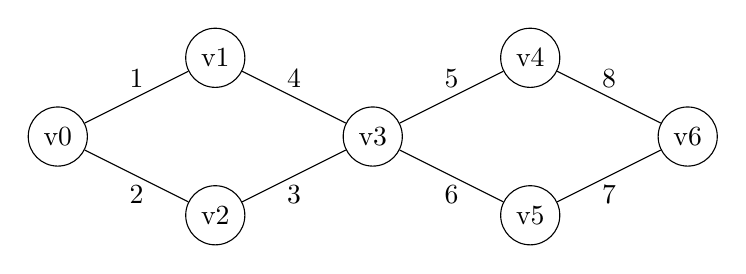
\begin{tikzpicture}[>=stealth']
			\node[circle,draw](v0)at(0,1){v0};
			\node[circle,draw](v1)at(2,2){v1};
			\node[circle,draw](v2)at(2,0){v2};
			\node[circle,draw](v3)at(4,1){v3};
			\node[circle,draw](v4)at(6,2){v4};
			\node[circle,draw](v5)at(6,0){v5};
			\node[circle,draw](v6)at(8,1){v6};
			\draw[above](v0)edge node{1}(v1);
			\draw[below](v0)edge node{2}(v2);
			\draw[above](v1)edge node{4}(v3);
			\draw[below](v2)edge node{3}(v3);
			\draw[above](v3)edge node{5}(v4);
			\draw[below](v3)edge node{6}(v5);
			\draw[above](v4)edge node{8}(v6);
			\draw[below](v5)edge node{7}(v6);
		\end{tikzpicture}
	\end{center}

	\subsection{邻接矩阵}
	$$
	\bbordermatrix{
			  &\rm v0&\rm v1&\rm v2&\rm v3&\rm v4&\rm v5&\rm v6\cr
		\rm v0&   0  &   1  &   1  &   0  &   0  &   0  &   0  \cr
		\rm v1&   1  &   0  &   0  &   1  &   0  &   0  &   0  \cr
		\rm v2&   1  &   0  &   0  &   1  &   0  &   0  &   0  \cr
		\rm v3&   0  &   1  &   1  &   0  &   1  &   1  &   0  \cr
		\rm v4&   0  &   0  &   0  &   1  &   0  &   0  &   1  \cr
		\rm v5&   0  &   0  &   0  &   1  &   0  &   0  &   1  \cr
		\rm v6&   0  &   0  &   0  &   0  &   1  &   1  &   0  \cr
	}
	$$

	\subsection{关联矩阵}
	$$
	\bbordermatrix{
			  &\rm 1&\rm 2&\rm 3&\rm 4&\rm 5&\rm 6&\rm 7&\rm 8\cr
		\rm v0&  1  &  1  &  0  &  0  &  0  &  0  &  0  &  0  \cr
		\rm v1&  1  &  0  &  0  &  1  &  0  &  0  &  0  &  0  \cr
		\rm v2&  0  &  1  &  1  &  0  &  0  &  0  &  0  &  0  \cr
		\rm v3&  0  &  0  &  1  &  1  &  1  &  1  &  0  &  0  \cr
		\rm v4&  0  &  0  &  0  &  0  &  1  &  0  &  0  &  1  \cr
		\rm v5&  0  &  0  &  0  &  0  &  0  &  1  &  1  &  0  \cr
		\rm v6&  0  &  0  &  0  &  0  &  0  &  0  &  1  &  1  \cr
	}
	$$

	\subsection{邻接表}
	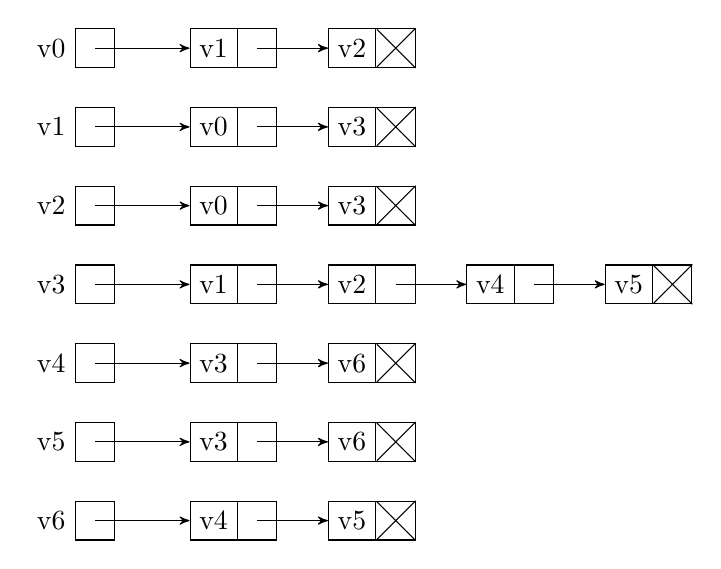
\begin{tikzpicture}[>=stealth',auto]
		\tikzstyle{listhead}=[rectangle,draw,minimum size=14pt];
		\tikzstyle{listnode}=[node distance=50pt,
			rectangle split,rectangle split horizontal,rectangle split parts=2,
			rectangle split part align=center,draw,minimum size=14pt,
			rectangle split empty part width=3pt];
		\node[listhead,label=left:v0](00){};
		\node[listnode,right of=00](01){v1}edge[<-](00.center);
		\node[listnode,right of=01](02){v2}edge[<-](01.two north|-01.two east);
		\draw(02.south east)--+(-14pt,+14pt)(02.north east)--+(-14pt,-14pt);

		\node[listhead,below of=00,label=left:v1](10){};
		\node[listnode,right of=10](11){v0}edge[<-](10.center);
		\node[listnode,right of=11](12){v3}edge[<-](11.two north|-11.two east);
		\draw(12.south east)--+(-14pt,+14pt)(12.north east)--+(-14pt,-14pt);

		\node[listhead,below of=10,label=left:v2](20){};
		\node[listnode,right of=20](21){v0}edge[<-](20.center);
		\node[listnode,right of=21](22){v3}edge[<-](21.two north|-21.two east);
		\draw(22.south east)--+(-14pt,+14pt)(22.north east)--+(-14pt,-14pt);

		\node[listhead,below of=20,label=left:v3](30){};
		\node[listnode,right of=30](31){v1}edge[<-](30.center);
		\node[listnode,right of=31](32){v2}edge[<-](31.two north|-31.two east);
		\node[listnode,right of=32](33){v4}edge[<-](32.two north|-32.two east);
		\node[listnode,right of=33](34){v5}edge[<-](33.two north|-33.two east);
		\draw(34.south east)--+(-14pt,+14pt)(34.north east)--+(-14pt,-14pt);

		\node[listhead,below of=30,label=left:v4](40){};
		\node[listnode,right of=40](41){v3}edge[<-](40.center);
		\node[listnode,right of=41](42){v6}edge[<-](41.two north|-41.two east);
		\draw(42.south east)--+(-14pt,+14pt)(42.north east)--+(-14pt,-14pt);

		\node[listhead,below of=40,label=left:v5](50){};
		\node[listnode,right of=50](51){v3}edge[<-](50.center);
		\node[listnode,right of=51](52){v6}edge[<-](51.two north|-51.two east);
		\draw(52.south east)--+(-14pt,+14pt)(52.north east)--+(-14pt,-14pt);

		\node[listhead,below of=50,label=left:v6](60){};
		\node[listnode,right of=60](61){v4}edge[<-](60.center);
		\node[listnode,right of=61](62){v5}edge[<-](61.two north|-61.two east);
		\draw(62.south east)--+(-14pt,+14pt)(62.north east)--+(-14pt,-14pt);
	\end{tikzpicture}

	\subsection{逆邻接表}
	同邻接表。
	
	\subsection{邻接多重表}
	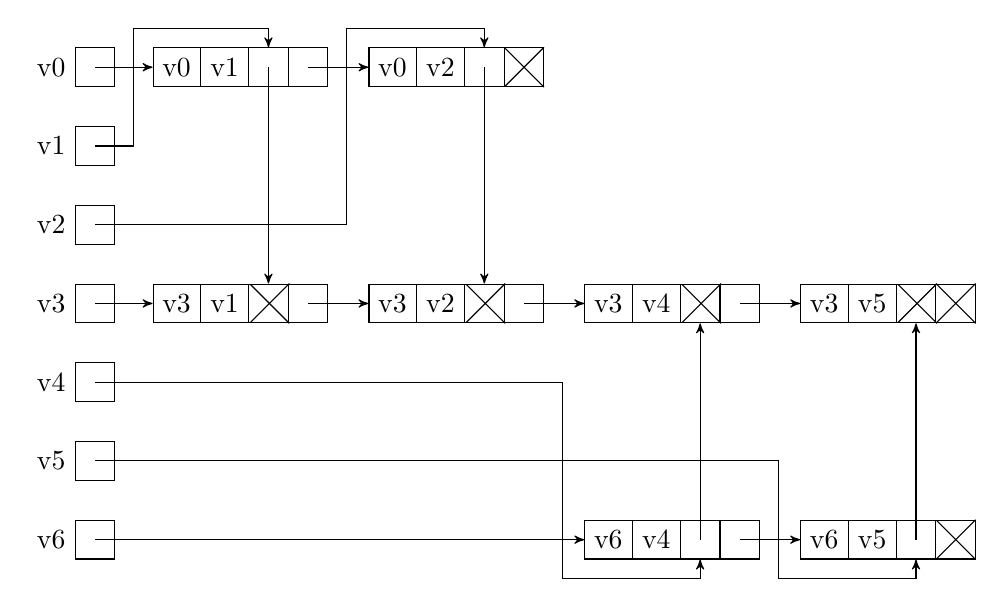
\begin{tikzpicture}[->,>=stealth',auto]
		\tikzstyle{listhead}=[rectangle,draw,minimum size=14pt];
		\tikzstyle{listnode}=[node distance=78pt,draw,
			rectangle split,rectangle split horizontal,rectangle split parts=4,
			rectangle split part align=center,minimum size=14pt,
			rectangle split empty part width=3pt];
		\tikzstyle{firstnode}=[listnode,node distance=52.5pt];
		\node[listhead,label=left:v0](0){};
		\node[firstnode,right of=0](01){v0\nodepart{two}v1};
		\node[listnode,right of=01](02){v0\nodepart{two}v2};
		\draw(0.center)--(01);
		\draw(01.four north|-01.four east)--(02);
		\draw[-](02.south east)--+(-14pt,+14pt)(02.north east)--+(-14pt,-14pt);

		\node[listhead,below of=0,label=left:v1](1){};
		\node[listhead,below of=1,label=left:v2](2){};

		\node[listhead,below of=2,label=left:v3](3){};
		\node[firstnode,right of=3](31){v3\nodepart{two}v1};
		\node[listnode,right of=31](32){v3\nodepart{two}v2};
		\node[listnode,right of=32](34){v3\nodepart{two}v4};
		\node[listnode,right of=34](35){v3\nodepart{two}v5};
		\draw(3.center)--(31);
		\draw(31.four north|-31.four east)--(32);
		\draw(32.four north|-32.four east)--(34);
		\draw(34.four north|-34.four east)--(35);
		\draw[-](35.south east)--+(-14pt,+14pt)(35.north east)--+(-14pt,-14pt);

		\node[listhead,below of=3,label=left:v4](4){};
		\node[listhead,below of=4,label=left:v5](5){};

		\node[listhead,below of=5,label=left:v6](6){};
		\node[firstnode,right of=6,draw=none](61){};
		\node[listnode,right of=61,draw=none](62){};
		\node[listnode,right of=62](64){v6\nodepart{two}v4};
		\node[listnode,right of=64](65){v6\nodepart{two}v5};
		\draw(6.center)--(64);
		\draw(64.four north|-64.four east)--(65);
		\draw[-](65.south east)--+(-14pt,+14pt)(65.north east)--+(-14pt,-14pt);

		\draw(1.center)-|+(14pt,42.5pt)-|(01.three north|-01.north east);
		\draw(01.three north|-01.three east)--(31.three north|-31.north east);
		\draw[-]([xshift=-14pt]31.south east)--+(-14pt,14pt)([xshift=-14pt]31.north east)--+(-14pt,-14pt);
		\draw(2.center)-|+(91pt,71pt)-|(02.three north|-02.north east);
		\draw(02.three north|-02.three east)--(32.three north|-32.north east);
		\draw[-]([xshift=-14pt]32.south east)--+(-14pt,14pt)([xshift=-14pt]32.north east)--+(-14pt,-14pt);

		\draw(4.center)-|+(169pt,-71pt)-|(64.three south|-64.south east);
		\draw(64.three south|-64.three east)--(34.three south|-34.south east);
		\draw[-]([xshift=-14pt]34.south east)--+(-14pt,14pt)([xshift=-14pt]34.north east)--+(-14pt,-14pt);
		\draw(5.center)-|+(247pt,-42.5pt)-|(65.three south|-65.south east);
		\draw(65.three south|-65.three east)--(35.three south|-35.south east);
		\draw[-]([xshift=-14pt]35.south east)--+(-14pt,14pt)([xshift=-14pt]35.north east)--+(-14pt,-14pt);
	\end{tikzpicture}

	\subsection{深度优先遍历}
	v0 $\to$ v1 $\to$ v3 $\to$ v2 $\to$ v4 $\to$ v6 $\to$ v5

	\subsection{广度优先遍历}
	v0 $\to$ v1 $\to$ v2 $\to$ v3 $\to$ v4 $\to$ v5 $\to$ v6

	\newpage
	\section{最小生成树}
	\begin{center}
		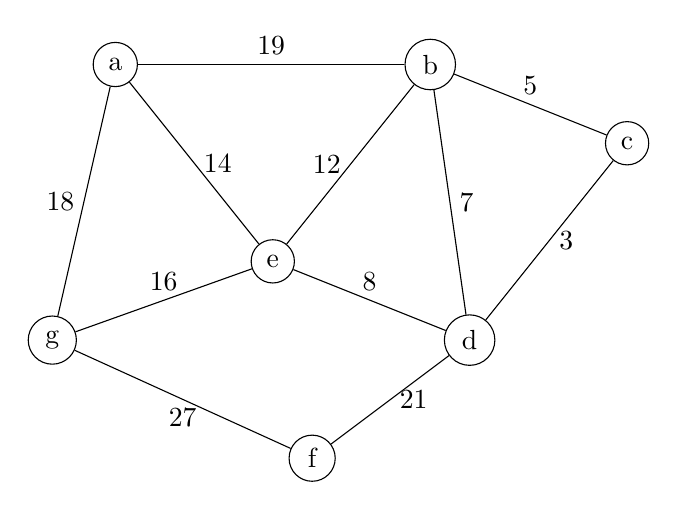
\begin{tikzpicture}[>=stealth']
			\node[circle,draw](a)at(1,5){a};
			\node[circle,draw](b)at(5,5){b};
			\node[circle,draw](c)at(7.5,4){c};
			\node[circle,draw](d)at(5.5,1.5){d};
			\node[circle,draw](e)at(3,2.5){e};
			\node[circle,draw](f)at(3.5,0){f};
			\node[circle,draw](g)at(.2,1.5){g};
			\draw[above](a)edge node{19}(b);
			\draw[right](a)edge node{14}(e);
			\draw[left](a)edge node{18}(g);
			\draw[above](b)edge node{5}(c);
			\draw[right](b)edge node{7}(d);
			\draw[left](b)edge node{12}(e);
			\draw[right](c)edge node{3}(d);
			\draw[above](d)edge node{8}(e);
			\draw[right](d)edge node{21}(f);
			\draw[above](e)edge node{16}(g);
			\draw[below](f)edge node{27}(g);
		\end{tikzpicture}
	\end{center}

	\subsection{Kruskal算法}
	\begin{center}
		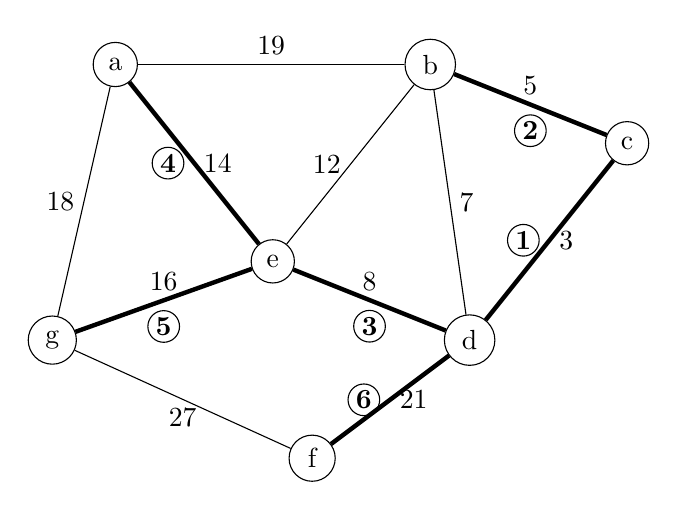
\begin{tikzpicture}[>=stealth']
			\node[circle,draw](a)at(1,5){a};
			\node[circle,draw](b)at(5,5){b};
			\node[circle,draw](c)at(7.5,4){c};
			\node[circle,draw](d)at(5.5,1.5){d};
			\node[circle,draw](e)at(3,2.5){e};
			\node[circle,draw](f)at(3.5,0){f};
			\node[circle,draw](g)at(.2,1.5){g};
			\draw[above](a)edge node{19}(b);
			\draw[right](a)edge node{14}(e);
			\draw[left](a)edge node{18}(g);
			\draw[above](b)edge node{5}(c);
			\draw[right](b)edge node{7}(d);
			\draw[left](b)edge node{12}(e);
			\draw[right](c)edge node{3}(d);
			\draw[above](d)edge node{8}(e);
			\draw[right](d)edge node{21}(f);
			\draw[above](e)edge node{16}(g);
			\draw[below](f)edge node{27}(g);
			\draw[ultra thick,left](c)edge node{\circled{1}}(d);
			\draw[ultra thick,below](b)edge node{\circled{2}}(c);
			\draw[ultra thick,below](d)edge node{\circled{3}}(e);
			\draw[ultra thick,left](a)edge node{\circled{4}}(e);
			\draw[ultra thick,below](e)edge node{\circled{5}}(g);
			\draw[ultra thick,left](d)edge node{\circled{6}}(f);
		\end{tikzpicture}
	\end{center}

	\subsection{Prim算法}
	\begin{center}
		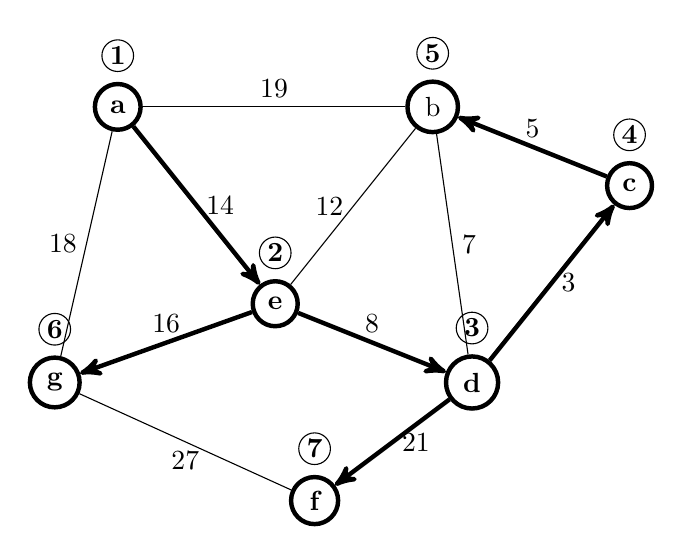
\begin{tikzpicture}[>=stealth']
			\tikzstyle{selected}=[circle,draw,ultra thick];
			\node[selected,label=\circled{1}](a)at(1,5){\bf a};
			\node[selected,label=\circled{5}](b)at(5,5){b};
			\node[selected,label=\circled{4}](c)at(7.5,4){\bf c};
			\node[selected,label=\circled{3}](d)at(5.5,1.5){\bf d};
			\node[selected,label=\circled{2}](e)at(3,2.5){\bf e};
			\node[selected,label=\circled{7}](f)at(3.5,0){\bf f};
			\node[selected,label=\circled{6}](g)at(.2,1.5){\bf g};
			\draw[above](a)edge node{19}(b);
			\draw[right](a)edge node{14}(e);
			\draw[left](a)edge node{18}(g);
			\draw[above](b)edge node{5}(c);
			\draw[right](b)edge node{7}(d);
			\draw[left](b)edge node{12}(e);
			\draw[right](c)edge node{3}(d);
			\draw[above](d)edge node{8}(e);
			\draw[right](d)edge node{21}(f);
			\draw[above](e)edge node{16}(g);
			\draw[below](f)edge node{27}(g);
			\draw[->,ultra thick](a)--(e);
			\draw[->,ultra thick](e)--(d);
			\draw[->,ultra thick](d)--(c);
			\draw[->,ultra thick](c)--(b);
			\draw[->,ultra thick](e)--(g);
			\draw[->,ultra thick](d)--(f);
		\end{tikzpicture}
	\end{center}

	\newpage
	\section{AOE图}
	\begin{center}
		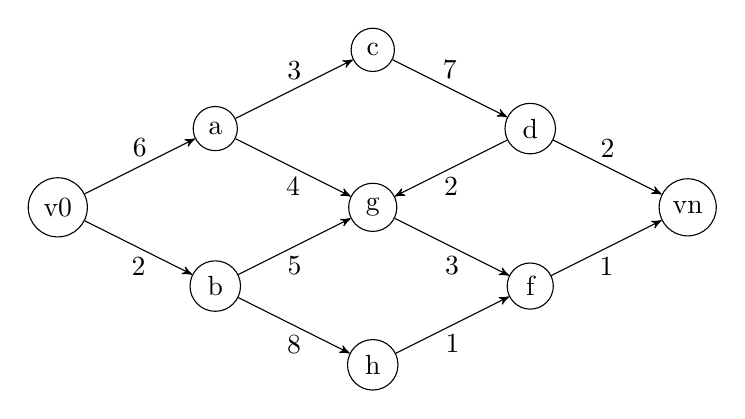
\begin{tikzpicture}[->,>=stealth']
			\node[draw,circle](v0)at(0,2){v0};
			\node[draw,circle](a)at(2,3){a};
			\node[draw,circle](b)at(2,1){b};
			\node[draw,circle](c)at(4,4){c};
			\node[draw,circle](g)at(4,2){g};
			\node[draw,circle](h)at(4,0){h};
			\node[draw,circle](d)at(6,3){d};
			\node[draw,circle](f)at(6,1){f};
			\node[draw,circle](vn)at(8,2){vn};
			\draw[above](v0)edge node{6}(a);
			\draw[below](v0)edge node{2}(b);
			\draw[above](a)edge node{3}(c);
			\draw[below](a)edge node{4}(g);
			\draw[below](b)edge node{5}(g);
			\draw[below](b)edge node{8}(h);
			\draw[above](c)edge node{7}(d);
			\draw[below](d)edge node{2}(g);
			\draw[below](g)edge node{3}(f);
			\draw[below](h)edge node{1}(f);
			\draw[above](d)edge node{2}(vn);
			\draw[below](f)edge node{1}(vn);
		\end{tikzpicture}
	\end{center}

	\subsection{拓扑有序序列}
	v0 $\to$ a $\to$ b $\to$ c $\to$ h $\to$ d $\to$ g $\to$ f $\to$ vn

	\subsection{关键路径}
	v0 $\to$ a $\to$ c $\to$ d $\to$ g $\to$ f $\to$ vn

	\section{广义表}
	令
	$$
	\begin{aligned}
		A&=(a,b)\\
		B&=(A,A)\\
		C&=(a,(b,A),B)\\
	\end{aligned}
	$$
	计算$\head A$和$\tail A$
	$$
	\begin{aligned}
		&\head A=a\\
		&\tail A=(b)\\
	\end{aligned}
	$$
	计算$\head\head\tail B$
	$$
	\begin{aligned}
		&\head\head\tail B\\
		=&\head\head(A)\\
		=&\head A\\
		=&a\\
	\end{aligned}
	$$
	计算$\tail\head\tail C$
	$$
	\begin{aligned}
		&\tail\head\tail C\\
		=&\tail\head((b,A),B)\\
		=&\tail(b,A)\\
		=&(A)
	\end{aligned}
	$$
\end{document}
